\begin{frame}
    \frametitle{Implementation for Lab CPU}
    \textbf{Type of interrupts:}
    \begin{itemize}
        \item Internal interrupts (non-maskable):
        \begin{itemize}
            \item ALU overflow
            \item Software interrupt through the \texttt{INT} instruction
        \end{itemize}
        \item External non-maskable interrupts:
        \begin{itemize}
            \item Lack of Voltage (Power Off)
            \item Special hardware line \texttt{cinm}
        \end{itemize}
        \item External maskable interrupts:
        \begin{itemize}
            \item 8 IO deivce interrupts
            \item Special hardware line \texttt{cintr} for all.
        \end{itemize}
    \end{itemize}
\end{frame}

\begin{frame}
    \frametitle{Implementation of IVT}
    \begin{table}[]
        \resizebox{0.9\textwidth}{!}{%
            \begin{tabular}{|c|c|c|}
                \hline
                \textbf{Address} & \textbf{Name} & \textbf{Type} \\ \hline
                0x0 & Reserved  & \multirow{3}{*}{Internal Interrupt} \\ \cline{1-2}
                0x1 & Software Interrupt (INT) & \\ \cline{1-2}
                0x2 & ALU Overflow & \\ \hline
                0x3 & Lack of Voltage (Power Off) & External Non-Maskable Interrupt \\ \hline
                0x4 & Level 0 & \multirow{8}{*}{External Maskable Interrupt} \\ \cline{1-2}
                0x5 & Level 1 & \\ \cline{1-2}
                0x6 & Level 2 & \\ \cline{1-2}
                0x7 & Level 3 & \\ \cline{1-2}
                0x8 & Level 4 & \\ \cline{1-2}
                0x9 & Level 5 & \\ \cline{1-2}
                0xA & Level 6 & \\ \cline{1-2}
                0xB & Level 7 & \\ \hline
            \end{tabular}
        }
    \end{table}
    \note{
    }

\end{frame}

\begin{frame}
    \frametitle{Interupt Instructions}
    The FR (Flag Register) will have a new bit \texttt{I} which will be used to enable or disable interrupts.
    The following instructions will be added:
    \begin{itemize}
        \item \texttt{EI} - Enable interrupts (sei)
        \item \texttt{DI} - Disable interrupts (cli)
        \item \texttt{INT} - Genrate software interrupt
        \item \texttt{RETI} - Return from interrupt
    \end{itemize}
\end{frame}

\begin{frame}
    \frametitle{Architecture}
    \begin{figure}
        \centering
        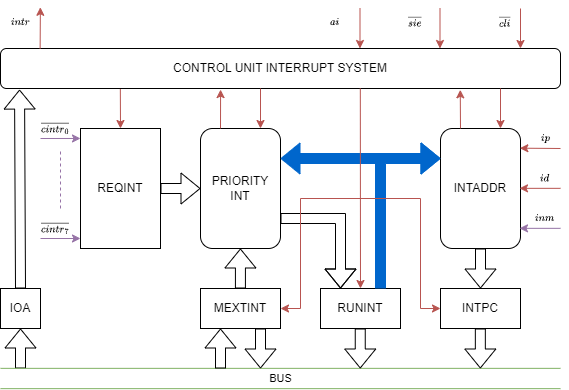
\includegraphics[width=0.8\textwidth]{media/isarchitecture.png}
    \end{figure}
\end{frame}

\begin{frame}
    \frametitle{Architecture Signals}
    \begin{itemize}
        \item $ip$ - Software Interrupt
        \item $id$ - ALU Overflow Interrupt
        \item $inm$ - external non-maskable interrupt (comes from $cinm$)
        \item $cintr_{i}$ - external maskable interrupt from device $i$
        \item $ai$ - external maskable interrupt active
        \item $intr$ - external maskable interrupt request to CPU
        \item $sie$/$cie$ - enable/disable external maskable interrupts
    \end{itemize}
\end{frame}

\begin{frame}
    \frametitle{Architecture Components}
    \begin{itemize}
        \item \texttt{REQINT} - Request external maskable interrupt register ($REQINT_{i} = 1$ means that the interrupt $i$ is requested)
        \item \texttt{MEXTINT} - Maskable external interrupt register ($MEXTINT_{i} = 1$ means that the interrupt $i$ is masked)
        \item \texttt{RUNINT} - Current running interrupts register ($RUNINT_{i} = 1$ means that the interrupt on level $i$ is running)
        \item \texttt{Priorrity INT} - Compute if the current interrupt has higher priority than the current running interrupt
        \item \texttt{INTADDR} - Compute the address of the ISR
        \item \texttt{INTPC} - The address for the current ISR
    \end{itemize}
\end{frame}

\begin{frame}
    \frametitle{External maskable interrupts Handling}
    \begin{enumerate}
        \item Verify for external maskable interrupt requests in the \texttt{REQINT} register.
        \item If there is one, verify if external maskable interrupts are enabled. (flag \texttt{I} in FR)
        \item If yes, filter the interrupts that are masked in the \texttt{MEXTINT} register.
        \item Find the highest priority interrupt that is not masked.
        \item Verify if it has higher priority than the current running interrupts in the \texttt{RUNINT} register:
        \item Send the interrupt to the CPU through the $intr$ signal.
        \item Wait for the CPU to acknowledge the interrupt. ($ai$ signal)
        \item Set the bit in the \texttt{RUNINT} register.
        \item Clear the bit in the \texttt{REQINT} register.
        \item Compute the address of the ISR and set the \texttt{INTPC} register.
    \end{enumerate}
\end{frame}

\begin{frame}
    \frametitle{External non-maskable interrupts Handling}
    \begin{enumerate}
        \item Verify for external non-maskable interrupt requests in the \texttt{inm} signal.
        \item Verify if there is no higher priority interrupt running.
        \item Compute the address of the ISR and set the \texttt{INTPC} register.
    \end{enumerate}
\end{frame}

\begin{frame}
    \frametitle{ALU Overflow Handling}
    \begin{enumerate}
        \item Verify for ALU overflow interrupt requests in the \texttt{id} signal.
        \item Verify if there is no higher priority interrupt running.
        \item Compute the address of the ISR and set the \texttt{INTPC} register.
        \item Inside the ISR, the CPU must clear the  overflow flag in the FR.
    \end{enumerate}
\end{frame}

\begin{frame}
    \frametitle{Software interrupts Handling}
    \begin{enumerate}
        \item Verify for software interrupt requests in the \texttt{ip} signal.
        \item There is no higher priority interrupt running.
        \item Compute the address of the ISR and set the \texttt{INTPC} register.
    \end{enumerate}
\end{frame}

\begin{frame}
    \frametitle{CPU acknowledge interrupts}
    \begin{enumerate}
        \item Save FR on the stack.
        \item Disable external maskable interrupts. (\texttt{EI} can be used to enable them back inside ISR)
        \item Save the current PC on the stack.
        \item Run the jump instruction from the \texttt{INTPC} register address.
    \end{enumerate}
\end{frame}

% \begin{frame}
%     \frametitle{Exam Questions}
%     Template: Having the following values in the registers at time 0,
%     interrupts requested with the time of the request and the type of the interrupt,
%     and how much time the CPU will take to handle every type of interrupt,
%     which is the order of the interrupts that will be handled by the CPU?
% \end{frame}


% \begin{frame}
%     \frametitle{Exam Questions}
%     \begin{table}[]
%         \begin{tabular}{|c|c|c|c|}
%             \hline
%             \texttt{REQINT} & \texttt{MEXTINT} & \texttt{RUNINT} & \texttt{FR} \\ \hline
%             0x00 & 0x00 & 0x00 & 0x00 \\ \hline
%         \end{tabular}
%     \end{table}

%     \begin{table}[]
%         \begin{tabular}{|c|c|c|c|}
%             \hline
%             Cycles from time 0 & Type of Request & Name \\ \hline
%             10 & External Maskable Interupt Level 5 & A \\ \hline
%             30 & External Maskable Interupt Level 3 & B \\ \hline
%             50 & External Maskable Interupt Level 7 & C \\ \hline
%             60 & External Maskable Interupt Level 1 & D \\ \hline
%             100 & External Non-Maskable Interupt & E \\ \hline
%             140 & ALU Overflow & F \\ \hline
%             150 & Software Interupt & G \\ \hline
%         \end{tabular}
%     \end{table}
% \end{frame}



% \begin{frame}
%     \frametitle{Exam Questions}
%     \begin{table}
%         \begin{tabular}{|c|c|c|c|}
%             \hline
%             Type of Request & Cycle to handle \\ \hline
%             External Maskable Interupt Level 0 & 30 \\ \hline
%             External Maskable Interupt Level 1 & 20 \\ \hline
%             External Maskable Interupt Level 2 & 10 \\ \hline
%             External Maskable Interupt Level 3 & 40 \\ \hline
%             External Maskable Interupt Level 4 & 20 \\ \hline
%             External Maskable Interupt Level 5 & 30 \\ \hline
%             External Maskable Interupt Level 6 & 10 \\ \hline
%             External Maskable Interupt Level 7 & 20 \\ \hline
%             External Non-Maskable Interupt & 5 \\ \hline
%             ALU Overflow & 10 \\ \hline
%             Software Interupt & 10 \\ \hline
%         \end{tabular}
%     \end{table}
% \end{frame}



% \begin{frame}
%     \frametitle{Exam Questions}
% \end{frame}